%%*************************************************************************
%%
%% PDDL 
%% V0.1
%% 2012/04/06
%% by Peter Boraros
%% See http://www.pborky.sk/contact for current contact information.
%%
%%*************************************************************************
%%
%% Legal Notice:
%%
%% This code is offered as-is without any warranty either expressed or
%% implied; without even the implied warranty of MERCHANTABILITY or
%% FITNESS FOR A PARTICULAR PURPOSE! 
%% User assumes all risk.
%%
%% This work by Peter Boraros is licensed under a 
%% Creative Commons Attribution-NonCommercial-ShareAlike 3.0 Unported License.
%% http://creativecommons.org/licenses/by-nc-sa/3.0/
%%
%%*************************************************************************


\documentclass[a4paper,journal]{IEEEtran}

\usepackage{cite}
% \usepackage[nocompress]{cite}
\usepackage{ifpdf}

\ifpdf
\usepackage[pdftex]{graphicx}
\graphicspath{{./img/}}
\DeclareGraphicsExtensions{.pdf}
\else
\usepackage[dvips]{graphicx}
\graphicspath{{./img/}}
\DeclareGraphicsExtensions{.eps}
\fi

\usepackage[cmex10]{amsmath}
\usepackage{amsfonts}
\usepackage{amssymb}
\interdisplaylinepenalty=2500

\usepackage{algorithmic}

\usepackage{array}

\usepackage{mdwmath}
\usepackage{mdwtab}

\usepackage{eqparbox}

\usepackage[hang,small,center,bf]{caption}
% \usepackage[tight,normalsize,sf,SF]{subfigure}
%\usepackage[tight,footnotesize]{subfigure}
\usepackage{subfig}
% \usepackage[caption=false,font=normalsize,labelfont=sf,textfont=sf]{subfig}
% \usepackage[caption=false,font=footnotesize]{subfig}
\usepackage[czech]{babel}
\usepackage[T1]{fontenc}
\usepackage[utf8x]{inputenc}
\usepackage{url}
\usepackage{fixltx2e}
\usepackage{stfloats}
\usepackage{ucs}
\usepackage{multirow}

% correct bad hyphenation here
\hyphenation{op-tical net-works semi-conduc-tor}

\renewcommand{\labelitemi}{$\bullet$}
\renewcommand{\labelitemii}{$\circ$}
\renewcommand{\labelitemiii}{$\ast$}

\setlength{\textheight}{260mm}

\begin{document}

\title{Pl\'anov\'an\'i a hry - PDDL}
\date{6.4.2012}
\author{Peter~Boráros %
\thanks{{Peter Boráros}, Czech technical university, Faculty of Electrical Engineering,
see~\texttt{http://www.pborky.sk/contact} for a contact infomation}}%

% The paper headers
%\markboth{Peter Boráros, Czech technical university, Faculty of Electrical Engineering, Prague, Czech Republic}{}

%\IEEEcompsoctitleabstractindextext{%
%\begin{abstract}
%
%\end{abstract}}

\maketitle
\IEEEdisplaynotcompsoctitleabstractindextext
\IEEEpeerreviewmaketitle

%krátký popis postupu formalizace plánovacího problému v PDDL
%seznam vybraných plánovačů
%parametry testovacího prostředí (native/virtual, OS, CPU, velikost paměti)
%graf doby výpočtu (srovnání doby výpočtu plánovačů na jednotlivých instancích problému)
%graf kvality řešení (srovnání cen nejlepších nalezených plánů na všech instancích problému)
%závěr – srovnání a vyhodnocení chování plánovačů (doba výpočtu, kvalita řešení) na základě naměřených hodnot

\section{Formalizace probl\'emu}

Predik\'aty:\\
\textbf{expert-mode} - robot je v expertnom mode\\
\textbf{advanced-mode} - robot pracuje v roz\v s\'irenom mode\\
\textbf{in-hand-board} - robot dr\v z\'i desku\\
\textbf{in-hand-saw} - robot dr\v z\'i pilu\\
\textbf{in-hand-paint} - robot dr\v z\'i \v st\v et\v ec\\
\textbf{hand-free}  - robot nedr\v z\'i nic\\
\textbf{at} - deska je na halde halde\\
\textbf{mounted} - deska je pripevnen\'a k stolu\\
\textbf{empty} - pracovne m\'isto je pr\'azdn\'e\\
\textbf{cuted} - deska je orezan\'a\\
\textbf{has-shape} - deska ma dan\'y tvar\\
\textbf{painted} - deska je natret\'a\\
\textbf{has-color} - deska ma danou barvu\\

Pr\'itomnos\v tn\'astroja / dosky v ruke robota je ur\v cen\'a  
predik\'atmi \texttt{in-hand}
a navy\v se  predik\'at \texttt{hand-free}
je pomocn\'y. Doska dalej mo\v ze by\v t primontovan\'a  - pred. \texttt{mounted} na konkr\'etnom pracovnom mieste
(mo\v zu byt 2 na jednom stole). Navy\v se pomocn\'y predik\'at \texttt{empty} hovor\'i\v ci je poz\'icia na stole je 
pr\'azdna. Po \'uprave dosky platia predik\'aty  \texttt{has-shape}, \texttt{has-color} a pomocn\'e
 \texttt{cuted},  \texttt{painted}. 
 Pri prechode do roz\v s\'iren\'eho / expertn\'eho m\'odu nastane platnos\v t axi\'omov \texttt{expert-mode} a 
 \texttt{advanced-mode}. 

\section{Pl\'anova\v ce}
Seznam vybran\'ych pl\'anova\v cu:
\begin{table}[!h]
\begin{center}
\begin{tabular}{|c|}\hline
fd-autotune-1 \\ \hline
lama2008 \\ \hline
roamer \\ \hline
\end{tabular}
\end{center}
\end{table} 

\section{Parametry testovac\'iho prostred\'i }
Bol pou\v zit\' y balik \texttt{signs.tgz} v nat\'ivnom prostred\'i Debian Wheezy x86\_64.



\section{Grafick\'e z\'avislosti}


\begin{table}[!h]
  \label{tbl:speed}
\caption{Z\'avislos\v t doby v\'ypo\v ctu (v sekund\'ach) od velikosti instance pre vybran\'e pl\'anova\v ce}
\begin{center}
\begin{tabular}{|c|c|c|c|c|c|}\hline
\textbf{planovac} / \textbf{vel. instance} & 2 & 3 & 4 & 5 & 6 \\ \hline
fd-autotune-1 & .087 & .196 & .975 & 4.289 & 24.047 \\ \hline
lama2008 & .091 & .652 & 1.805 & 22.358 & 67.804 \\ \hline
roamer & .098 & .743 & 4.198 & 37.046 & 343.356 \\ \hline
\end{tabular}
\end{center}
\end{table}

\begin{figure}[h]%
  \centering
  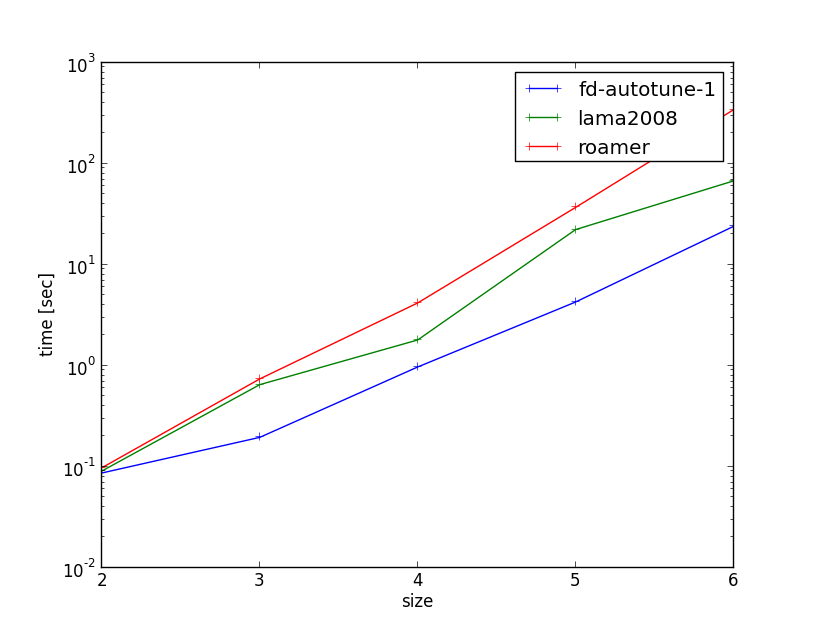
\includegraphics[width=80mm]{speed}
  \caption{Graf z\'avislosti r\'ychlosti rie\v senia od ve\v lkosti in\v stance}
  \label{fig:speed}
\end{figure}
\begin{figure}[h]%
  \centering
  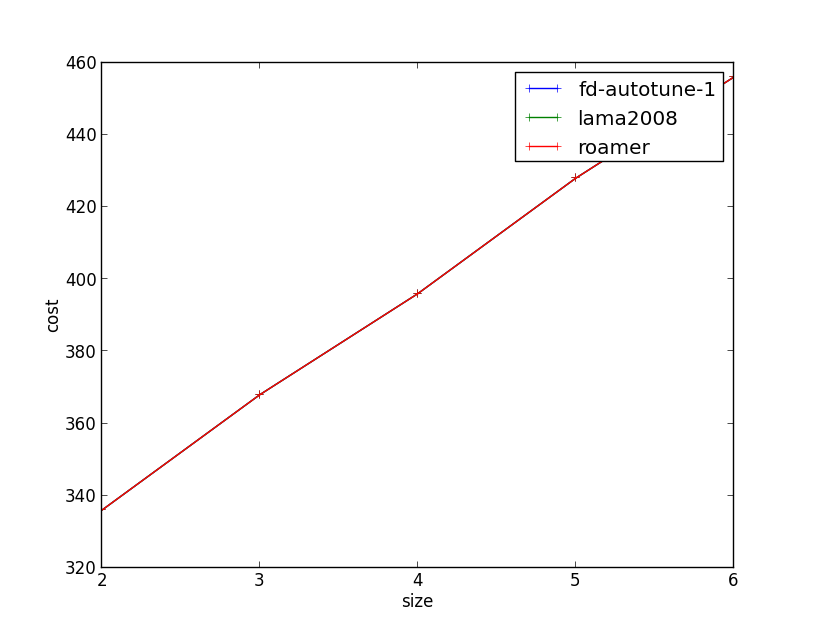
\includegraphics[width=80mm]{qual}
  \caption{Graf z\'avislosti ceny rie\v senia od ve\v lkosti in\v stancie (v\v sechny pl\'anova\v ce na\v sli \v re\v sen\'i se stejnou cenou)}
  \label{fig:qual}
\end{figure}
%
%\section{Graf kvality \v re\v sen\'i}
\section{Z\'av\v er}
 Ako metriku kvality pl\'anova\v ca je mo\v zne pou\v zi\v t funckiu odvoden\'u od ceny najlep\v sieho n\'ajden\'eho rie\v senia. Takouto funkciou by mohla by\v t
 $f_x = \frac{1}{\left|{Y}\right|}\sum_{y \in Y} \frac{p_{x,y}}{p_{ymin}}$, kde $f_x$ je kvalita pl\'anova\v ca $x$, $Y$ je mno\v zina kardinal\'it testovan\'ych in\v stanci\'i, 
 $p_{x,y}$ je cena najlep\v sieho rie\v senia pl\'anova\v ca $x$ pri kardinalite in\v stancie $y$ a $p_{ymin}$ je najlep\v sia mo\v zn\'a cena rie\v senia
 pri kardinalite $y$. Nev\'yhoda takejto metriky je obtia\v znos\v t ur\v cenia  $p_{ymin}$. Pre zafixovan\'u ve\v lkos\v t instancie $k$ je mo\v zn\'e priamo porovna\v t
 hodnoty $p_{x,k}$.
 
 Na obr. \ref{fig:qual} je z\'avislos\v t ceny najlep\v sieho rie\v senia od ve\v lkosti in\v stancie pre jednotliv\'e pl\'anova\v ce.
 S oh\v ladom na toto krit\'erium, pl\'anova\v ce dosiahli rovnak\'ych v\'ysledkov.
 V tab.~1 a na  obr.~\ref{fig:speed} je z\'avislos\v t doby v\'ypo\v ctu od ve\v lkosti in\v stancie. Grafick\'a z\'avislos\v t je v semilogaritmickej 
 mierke. V tomto experimente bol najr\'ychle\v s\'im pl\'anova\v c \texttt{fd-autotune-1} a najpomal\v s\'im \texttt{roamer}, no nutn\'e podotkn\'u\v t, 
 \v ze napriek tomu sa na tejto malej vzorke jav\'i, \v ze aymptotick\'a zlo\v zitos\v t \v ziadneho z nich, nie je lep\v sia ako $O(e^n)$.
 
 
 

%


% that's all folks
\end{document}
